\documentclass[twoside]{book}

% Packages required by doxygen
\usepackage{fixltx2e}
\usepackage{calc}
\usepackage{doxygen}
\usepackage[export]{adjustbox} % also loads graphicx
\usepackage{graphicx}
\usepackage[utf8]{inputenc}
\usepackage{makeidx}
\usepackage{multicol}
\usepackage{multirow}
\PassOptionsToPackage{warn}{textcomp}
\usepackage{textcomp}
\usepackage[nointegrals]{wasysym}
\usepackage[table]{xcolor}

% Font selection
\usepackage[T1]{fontenc}
\usepackage[scaled=.90]{helvet}
\usepackage{courier}
\usepackage{amssymb}
\usepackage{sectsty}
\renewcommand{\familydefault}{\sfdefault}
\allsectionsfont{%
  \fontseries{bc}\selectfont%
  \color{darkgray}%
}
\renewcommand{\DoxyLabelFont}{%
  \fontseries{bc}\selectfont%
  \color{darkgray}%
}
\newcommand{\+}{\discretionary{\mbox{\scriptsize$\hookleftarrow$}}{}{}}

% Page & text layout
\usepackage{geometry}
\geometry{%
  a4paper,%
  top=2.5cm,%
  bottom=2.5cm,%
  left=2.5cm,%
  right=2.5cm%
}
\tolerance=750
\hfuzz=15pt
\hbadness=750
\setlength{\emergencystretch}{15pt}
\setlength{\parindent}{0cm}
\setlength{\parskip}{3ex plus 2ex minus 2ex}
\makeatletter
\renewcommand{\paragraph}{%
  \@startsection{paragraph}{4}{0ex}{-1.0ex}{1.0ex}{%
    \normalfont\normalsize\bfseries\SS@parafont%
  }%
}
\renewcommand{\subparagraph}{%
  \@startsection{subparagraph}{5}{0ex}{-1.0ex}{1.0ex}{%
    \normalfont\normalsize\bfseries\SS@subparafont%
  }%
}
\makeatother

% Headers & footers
\usepackage{fancyhdr}
\pagestyle{fancyplain}
\fancyhead[LE]{\fancyplain{}{\bfseries\thepage}}
\fancyhead[CE]{\fancyplain{}{}}
\fancyhead[RE]{\fancyplain{}{\bfseries\leftmark}}
\fancyhead[LO]{\fancyplain{}{\bfseries\rightmark}}
\fancyhead[CO]{\fancyplain{}{}}
\fancyhead[RO]{\fancyplain{}{\bfseries\thepage}}
\fancyfoot[LE]{\fancyplain{}{}}
\fancyfoot[CE]{\fancyplain{}{}}
\fancyfoot[RE]{\fancyplain{}{\bfseries\scriptsize Generated by Doxygen }}
\fancyfoot[LO]{\fancyplain{}{\bfseries\scriptsize Generated by Doxygen }}
\fancyfoot[CO]{\fancyplain{}{}}
\fancyfoot[RO]{\fancyplain{}{}}
\renewcommand{\footrulewidth}{0.4pt}
\renewcommand{\chaptermark}[1]{%
  \markboth{#1}{}%
}
\renewcommand{\sectionmark}[1]{%
  \markright{\thesection\ #1}%
}

% Indices & bibliography
\usepackage{natbib}
\usepackage[titles]{tocloft}
\setcounter{tocdepth}{3}
\setcounter{secnumdepth}{5}
\makeindex

% Hyperlinks (required, but should be loaded last)
\usepackage{ifpdf}
\ifpdf
  \usepackage[pdftex,pagebackref=true]{hyperref}
\else
  \usepackage[ps2pdf,pagebackref=true]{hyperref}
\fi
\hypersetup{%
  colorlinks=true,%
  linkcolor=blue,%
  citecolor=blue,%
  unicode%
}

% Custom commands
\newcommand{\clearemptydoublepage}{%
  \newpage{\pagestyle{empty}\cleardoublepage}%
}

\usepackage{caption}
\captionsetup{labelsep=space,justification=centering,font={bf},singlelinecheck=off,skip=4pt,position=top}

%===== C O N T E N T S =====

\begin{document}

% Titlepage & ToC
\hypersetup{pageanchor=false,
             bookmarksnumbered=true,
             pdfencoding=unicode
            }
\pagenumbering{roman}
\begin{titlepage}
\vspace*{7cm}
\begin{center}%
{\Large QT Client Consumer \\[1ex]\large 0.\+0.\+1 }\\
\vspace*{1cm}
{\large Generated by Doxygen 1.8.11}\\
\end{center}
\end{titlepage}
\clearemptydoublepage
\tableofcontents
\clearemptydoublepage
\pagenumbering{arabic}
\hypersetup{pageanchor=true}

%--- Begin generated contents ---
\chapter{Namespace Index}
\section{Lista de namespaces}
Lista dos namespaces com uma breve descrição\+:\begin{DoxyCompactList}
\item\contentsline{section}{\hyperlink{namespace_ui}{Ui} }{\pageref{namespace_ui}}{}
\end{DoxyCompactList}

\chapter{Hierarchical Index}
\section{Class Hierarchy}
This inheritance list is sorted roughly, but not completely, alphabetically\+:\begin{DoxyCompactList}
\item Q\+Main\+Window\begin{DoxyCompactList}
\item \contentsline{section}{Main\+Window}{\pageref{class_main_window}}{}
\end{DoxyCompactList}
\end{DoxyCompactList}

\chapter{Class Index}
\section{Lista de componentes}
Lista de classes, estruturas, uniões e interfaces com uma breve descrição\+:\begin{DoxyCompactList}
\item\contentsline{section}{\hyperlink{class_main_window}{Main\+Window} \\*A classe \hyperlink{class_main_window}{Main\+Window} representa o contâiner da janela da aplicação e seus componentes }{\pageref{class_main_window}}{}
\item\contentsline{section}{\hyperlink{class_plotter}{Plotter} }{\pageref{class_plotter}}{}
\end{DoxyCompactList}

\chapter{File Index}
\section{Lista de ficheiros}
Lista de todos os ficheiros com uma breve descrição\+:\begin{DoxyCompactList}
\item\contentsline{section}{\hyperlink{main_8cpp}{main.\+cpp} }{\pageref{main_8cpp}}{}
\item\contentsline{section}{\hyperlink{mainwindow_8cpp}{mainwindow.\+cpp} }{\pageref{mainwindow_8cpp}}{}
\item\contentsline{section}{\hyperlink{mainwindow_8h}{mainwindow.\+h} }{\pageref{mainwindow_8h}}{}
\item\contentsline{section}{\hyperlink{plotter_8cpp}{plotter.\+cpp} }{\pageref{plotter_8cpp}}{}
\item\contentsline{section}{\hyperlink{plotter_8h}{plotter.\+h} }{\pageref{plotter_8h}}{}
\end{DoxyCompactList}

\chapter{Namespace Documentation}
\hypertarget{namespace_ui}{}\section{Ui Namespace Reference}
\label{namespace_ui}\index{Ui@{Ui}}
\subsection*{Classes}
\begin{DoxyCompactItemize}
\item 
class \hyperlink{class_ui_1_1_main_window}{Main\+Window}
\end{DoxyCompactItemize}

\chapter{Class Documentation}
\hypertarget{class_main_window}{}\section{Main\+Window Class Reference}
\label{class_main_window}\index{Main\+Window@{Main\+Window}}


{\ttfamily \#include $<$mainwindow.\+h$>$}



Inheritance diagram for Main\+Window\+:
\nopagebreak
\begin{figure}[H]
\begin{center}
\leavevmode
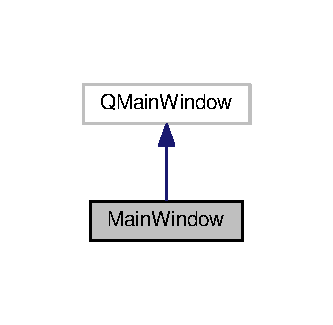
\includegraphics[width=160pt]{class_main_window__inherit__graph}
\end{center}
\end{figure}


Collaboration diagram for Main\+Window\+:
\nopagebreak
\begin{figure}[H]
\begin{center}
\leavevmode
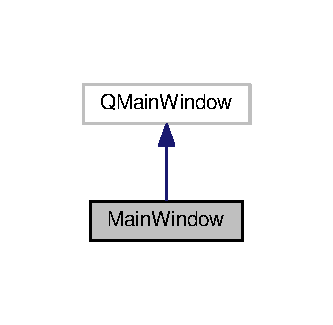
\includegraphics[width=160pt]{class_main_window__coll__graph}
\end{center}
\end{figure}
\subsection*{Public Slots}
\begin{DoxyCompactItemize}
\item 
void \hyperlink{class_main_window_a0edca0c59fb238bea02b248c90b89698}{show\+Message} (Q\+String msg)
\end{DoxyCompactItemize}
\subsection*{Public Member Functions}
\begin{DoxyCompactItemize}
\item 
\hyperlink{class_main_window_a8b244be8b7b7db1b08de2a2acb9409db}{Main\+Window} (Q\+Widget $\ast$parent=0)
\item 
\hyperlink{class_main_window_ae98d00a93bc118200eeef9f9bba1dba7}{$\sim$\+Main\+Window} ()
\end{DoxyCompactItemize}


\subsection{Constructor \& Destructor Documentation}
\index{Main\+Window@{Main\+Window}!Main\+Window@{Main\+Window}}
\index{Main\+Window@{Main\+Window}!Main\+Window@{Main\+Window}}
\subsubsection[{\texorpdfstring{Main\+Window(\+Q\+Widget $\ast$parent=0)}{MainWindow(QWidget *parent=0)}}]{\setlength{\rightskip}{0pt plus 5cm}Main\+Window\+::\+Main\+Window (
\begin{DoxyParamCaption}
\item[{Q\+Widget $\ast$}]{parent = {\ttfamily 0}}
\end{DoxyParamCaption}
)\hspace{0.3cm}{\ttfamily [explicit]}}\hypertarget{class_main_window_a8b244be8b7b7db1b08de2a2acb9409db}{}\label{class_main_window_a8b244be8b7b7db1b08de2a2acb9409db}
\index{Main\+Window@{Main\+Window}!````~Main\+Window@{$\sim$\+Main\+Window}}
\index{````~Main\+Window@{$\sim$\+Main\+Window}!Main\+Window@{Main\+Window}}
\subsubsection[{\texorpdfstring{$\sim$\+Main\+Window()}{~MainWindow()}}]{\setlength{\rightskip}{0pt plus 5cm}Main\+Window\+::$\sim$\+Main\+Window (
\begin{DoxyParamCaption}
{}
\end{DoxyParamCaption}
)}\hypertarget{class_main_window_ae98d00a93bc118200eeef9f9bba1dba7}{}\label{class_main_window_ae98d00a93bc118200eeef9f9bba1dba7}


\subsection{Member Function Documentation}
\index{Main\+Window@{Main\+Window}!show\+Message@{show\+Message}}
\index{show\+Message@{show\+Message}!Main\+Window@{Main\+Window}}
\subsubsection[{\texorpdfstring{show\+Message}{showMessage}}]{\setlength{\rightskip}{0pt plus 5cm}void Main\+Window\+::show\+Message (
\begin{DoxyParamCaption}
\item[{Q\+String}]{msg}
\end{DoxyParamCaption}
)\hspace{0.3cm}{\ttfamily [slot]}}\hypertarget{class_main_window_a0edca0c59fb238bea02b248c90b89698}{}\label{class_main_window_a0edca0c59fb238bea02b248c90b89698}


The documentation for this class was generated from the following files\+:\begin{DoxyCompactItemize}
\item 
Qt\+Tcp\+Server/\hyperlink{mainwindow_8h}{mainwindow.\+h}\item 
Qt\+Tcp\+Server/\hyperlink{mainwindow_8cpp}{mainwindow.\+cpp}\end{DoxyCompactItemize}

\hypertarget{class_plotter}{}\section{Plotter Class Reference}
\label{class_plotter}\index{Plotter@{Plotter}}


{\ttfamily \#include $<$plotter.\+h$>$}



Inheritance diagram for Plotter\+:
\nopagebreak
\begin{figure}[H]
\begin{center}
\leavevmode
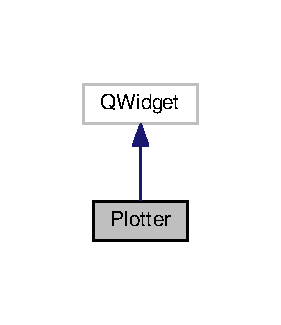
\includegraphics[width=135pt]{class_plotter__inherit__graph}
\end{center}
\end{figure}


Collaboration diagram for Plotter\+:
\nopagebreak
\begin{figure}[H]
\begin{center}
\leavevmode
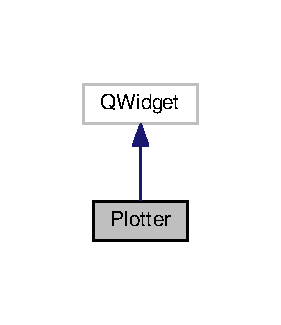
\includegraphics[width=135pt]{class_plotter__coll__graph}
\end{center}
\end{figure}
\subsection*{Public Member Functions}
\begin{DoxyCompactItemize}
\item 
\hyperlink{class_plotter_a367b6890c36910a27ec710ac3693e64b}{Plotter} (Q\+Widget $\ast$parent=0)
\begin{DoxyCompactList}\small\item\em Construtor do componente \hyperlink{class_plotter}{Plotter}. \end{DoxyCompactList}\item 
void \hyperlink{class_plotter_ac4341569909943e37e1ff756587e6e12}{paint\+Event} (Q\+Paint\+Event $\ast$e)
\begin{DoxyCompactList}\small\item\em Paint event. \end{DoxyCompactList}\item 
void \hyperlink{class_plotter_ae73b5093b98bbbebd6abdb4e7e7807ed}{load\+Data} (std\+::vector$<$ double $>$, std\+::vector$<$ double $>$)
\begin{DoxyCompactList}\small\item\em Função que carrega os dados referentes aos tempos e aos dados. \end{DoxyCompactList}\end{DoxyCompactItemize}


\subsection{Constructor \& Destructor Documentation}
\index{Plotter@{Plotter}!Plotter@{Plotter}}
\index{Plotter@{Plotter}!Plotter@{Plotter}}
\subsubsection[{\texorpdfstring{Plotter(\+Q\+Widget $\ast$parent=0)}{Plotter(QWidget *parent=0)}}]{\setlength{\rightskip}{0pt plus 5cm}Plotter\+::\+Plotter (
\begin{DoxyParamCaption}
\item[{Q\+Widget $\ast$}]{parent = {\ttfamily 0}}
\end{DoxyParamCaption}
)\hspace{0.3cm}{\ttfamily [explicit]}}\hypertarget{class_plotter_a367b6890c36910a27ec710ac3693e64b}{}\label{class_plotter_a367b6890c36910a27ec710ac3693e64b}


Construtor do componente \hyperlink{class_plotter}{Plotter}. 

adiciona os valores aos vectores de tempos e de dados 

\subsection{Member Function Documentation}
\index{Plotter@{Plotter}!load\+Data@{load\+Data}}
\index{load\+Data@{load\+Data}!Plotter@{Plotter}}
\subsubsection[{\texorpdfstring{load\+Data(std\+::vector$<$ double $>$, std\+::vector$<$ double $>$)}{loadData(std::vector< double >, std::vector< double >)}}]{\setlength{\rightskip}{0pt plus 5cm}void Plotter\+::load\+Data (
\begin{DoxyParamCaption}
\item[{std\+::vector$<$ double $>$}]{t, }
\item[{std\+::vector$<$ double $>$}]{d}
\end{DoxyParamCaption}
)}\hypertarget{class_plotter_ae73b5093b98bbbebd6abdb4e7e7807ed}{}\label{class_plotter_ae73b5093b98bbbebd6abdb4e7e7807ed}


Função que carrega os dados referentes aos tempos e aos dados. 

Recebe os 30 ultimos dados e os usa na classe \hyperlink{class_plotter}{Plotter}. \index{Plotter@{Plotter}!paint\+Event@{paint\+Event}}
\index{paint\+Event@{paint\+Event}!Plotter@{Plotter}}
\subsubsection[{\texorpdfstring{paint\+Event(\+Q\+Paint\+Event $\ast$e)}{paintEvent(QPaintEvent *e)}}]{\setlength{\rightskip}{0pt plus 5cm}void Plotter\+::paint\+Event (
\begin{DoxyParamCaption}
\item[{Q\+Paint\+Event $\ast$}]{e}
\end{DoxyParamCaption}
)}\hypertarget{class_plotter_ac4341569909943e37e1ff756587e6e12}{}\label{class_plotter_ac4341569909943e37e1ff756587e6e12}


Paint event. 

Desenha o grafico utilizando retas, usando dois pontos de cada vez. 

The documentation for this class was generated from the following files\+:\begin{DoxyCompactItemize}
\item 
\hyperlink{plotter_8h}{plotter.\+h}\item 
\hyperlink{plotter_8cpp}{plotter.\+cpp}\end{DoxyCompactItemize}

\chapter{File Documentation}
\hypertarget{main_8cpp}{}\section{Referência ao ficheiro main.\+cpp}
\label{main_8cpp}\index{main.\+cpp@{main.\+cpp}}
{\ttfamily \#include \char`\"{}mainwindow.\+h\char`\"{}}\newline
{\ttfamily \#include $<$Q\+Application$>$}\newline
\subsection*{Funções}
\begin{DoxyCompactItemize}
\item 
int \hyperlink{main_8cpp_a0ddf1224851353fc92bfbff6f499fa97}{main} (int argc, char $\ast$argv\mbox{[}$\,$\mbox{]})
\end{DoxyCompactItemize}


\subsection{Documentação das funções}
\mbox{\Hypertarget{main_8cpp_a0ddf1224851353fc92bfbff6f499fa97}\label{main_8cpp_a0ddf1224851353fc92bfbff6f499fa97}} 
\index{main.\+cpp@{main.\+cpp}!main@{main}}
\index{main@{main}!main.\+cpp@{main.\+cpp}}
\subsubsection{\texorpdfstring{main()}{main()}}
{\footnotesize\ttfamily int main (\begin{DoxyParamCaption}\item[{int}]{argc,  }\item[{char $\ast$}]{argv\mbox{[}$\,$\mbox{]} }\end{DoxyParamCaption})}


\hypertarget{mainwindow_8cpp}{}\section{Qt\+Tcp\+Server/mainwindow.cpp File Reference}
\label{mainwindow_8cpp}\index{Qt\+Tcp\+Server/mainwindow.\+cpp@{Qt\+Tcp\+Server/mainwindow.\+cpp}}
{\ttfamily \#include \char`\"{}mainwindow.\+h\char`\"{}}\\*
{\ttfamily \#include \char`\"{}ui\+\_\+mainwindow.\+h\char`\"{}}\\*
{\ttfamily \#include \char`\"{}myserver.\+h\char`\"{}}\\*
{\ttfamily \#include $<$Q\+String\+List$>$}\\*
Include dependency graph for mainwindow.\+cpp\+:
\nopagebreak
\begin{figure}[H]
\begin{center}
\leavevmode
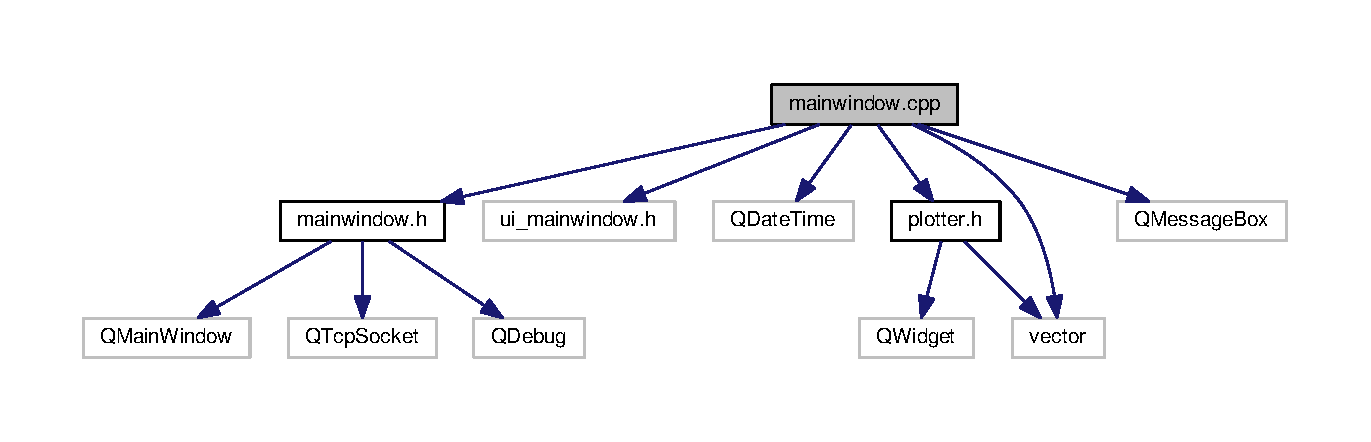
\includegraphics[width=350pt]{mainwindow_8cpp__incl}
\end{center}
\end{figure}

\hypertarget{mainwindow_8h}{}\section{Qt\+Tcp\+Client\+Producer/mainwindow.h File Reference}
\label{mainwindow_8h}\index{Qt\+Tcp\+Client\+Producer/mainwindow.\+h@{Qt\+Tcp\+Client\+Producer/mainwindow.\+h}}
{\ttfamily \#include $<$Q\+Main\+Window$>$}\\*
{\ttfamily \#include $<$Q\+Tcp\+Socket$>$}\\*
{\ttfamily \#include $<$Q\+Debug$>$}\\*
{\ttfamily \#include $<$Q\+String$>$}\\*
Include dependency graph for mainwindow.\+h\+:
\nopagebreak
\begin{figure}[H]
\begin{center}
\leavevmode
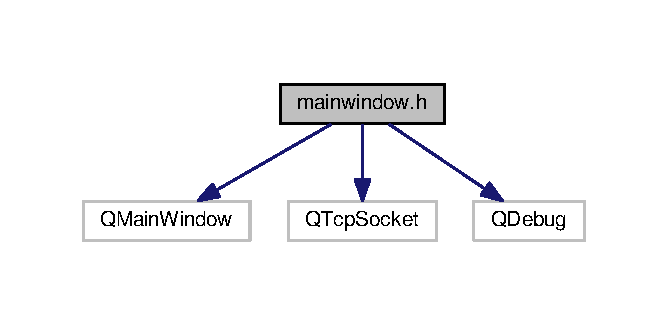
\includegraphics[width=350pt]{mainwindow_8h__incl}
\end{center}
\end{figure}
This graph shows which files directly or indirectly include this file\+:
\nopagebreak
\begin{figure}[H]
\begin{center}
\leavevmode
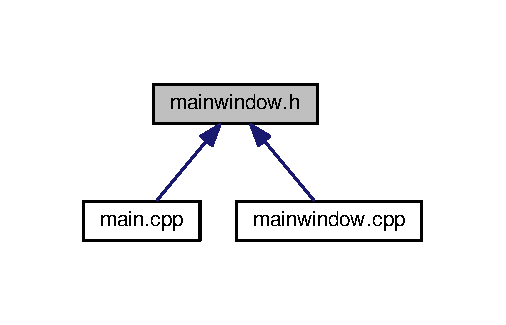
\includegraphics[width=314pt]{mainwindow_8h__dep__incl}
\end{center}
\end{figure}
\subsection*{Classes}
\begin{DoxyCompactItemize}
\item 
class \hyperlink{class_main_window}{Main\+Window}
\begin{DoxyCompactList}\small\item\em A classe \hyperlink{class_main_window}{Main\+Window} representa o contâiner da janela da aplicação e seus componentes. \end{DoxyCompactList}\end{DoxyCompactItemize}
\subsection*{Namespaces}
\begin{DoxyCompactItemize}
\item 
 \hyperlink{namespace_ui}{Ui}
\end{DoxyCompactItemize}

\hypertarget{plotter_8cpp}{}\section{plotter.\+cpp File Reference}
\label{plotter_8cpp}\index{plotter.\+cpp@{plotter.\+cpp}}
{\ttfamily \#include \char`\"{}plotter.\+h\char`\"{}}\\*
{\ttfamily \#include $<$Q\+Painter$>$}\\*
{\ttfamily \#include $<$Q\+Brush$>$}\\*
{\ttfamily \#include $<$Q\+Pen$>$}\\*
{\ttfamily \#include $<$Q\+Color$>$}\\*
{\ttfamily \#include $<$cmath$>$}\\*
{\ttfamily \#include $<$Q\+Debug$>$}\\*
Include dependency graph for plotter.\+cpp\+:
\nopagebreak
\begin{figure}[H]
\begin{center}
\leavevmode
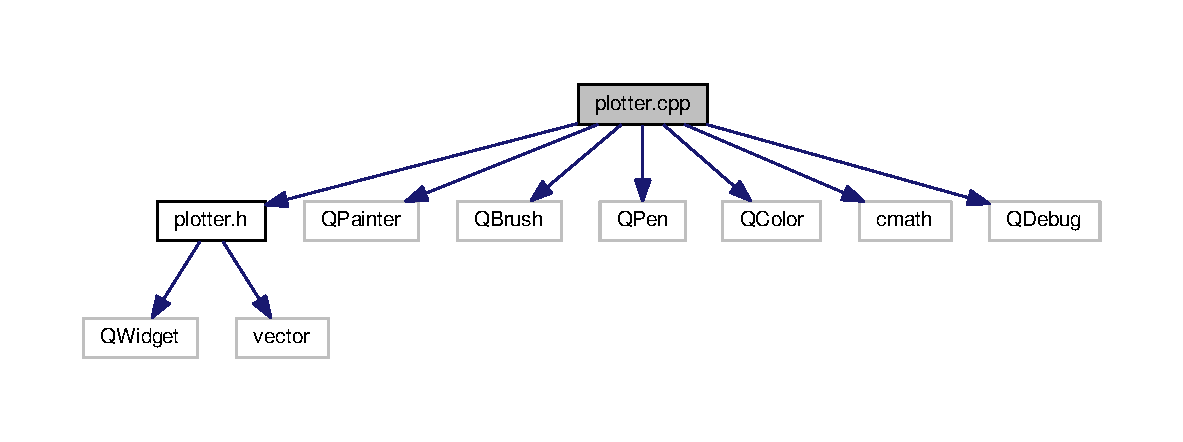
\includegraphics[width=350pt]{plotter_8cpp__incl}
\end{center}
\end{figure}

\hypertarget{plotter_8h}{}\section{plotter.\+h File Reference}
\label{plotter_8h}\index{plotter.\+h@{plotter.\+h}}
{\ttfamily \#include $<$Q\+Widget$>$}\\*
{\ttfamily \#include $<$vector$>$}\\*
Include dependency graph for plotter.\+h\+:
\nopagebreak
\begin{figure}[H]
\begin{center}
\leavevmode
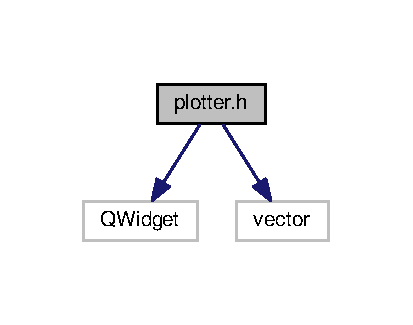
\includegraphics[width=198pt]{plotter_8h__incl}
\end{center}
\end{figure}
This graph shows which files directly or indirectly include this file\+:
\nopagebreak
\begin{figure}[H]
\begin{center}
\leavevmode
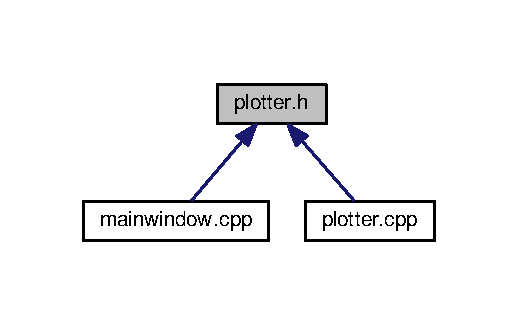
\includegraphics[width=249pt]{plotter_8h__dep__incl}
\end{center}
\end{figure}
\subsection*{Classes}
\begin{DoxyCompactItemize}
\item 
class \hyperlink{class_plotter}{Plotter}
\end{DoxyCompactItemize}

%--- End generated contents ---

% Index
\backmatter
\newpage
\phantomsection
\clearemptydoublepage
\addcontentsline{toc}{chapter}{Index}
\printindex

\end{document}
